\section{Methods}

The 

Conceptually these systems are quite simple to model,
consisting of binary spins which can either have the value 1 (up) or -1 (down).
The energy of this system is given by summing up nearest neighbour spins of all
spins in our system. We evolve our system by randomly selecting spins and
changing their values if it is energetically favourable for the system. To not
have our system being stuck in the ground state (lowest energy state) we will randomly flip some spins
anyway even if it is not energetically favourable, this behaviour is actually
something for real systems to. 
\subsection{Ising model}
The Ising model, without an external magnetic field, is given by
\cref{eq:ising}, where $E_i$ is the energy of a given microstate s$_k$ and s$_l$ takes values of $\pm 1$, N is the
number of spins, J is a coupling constant corresponding to the strength of the
interaction between the neighbouring spins and $<kl>$ means that we are sum over
nearest neighbour only. 

\begin{equation}
  \label{eq:ising}
  E_i = -J\sum_{<kl>}^{L^2} s_k s_l
\end{equation}

We will
use quadratic grids with grid width L and periodic
boundary conditions.



\subsection{Metropolis algorithm}

The Metropolis algorithm is a 



Since the Ising model is a binary system the number of possible microstates is
2$^{L^2}$. Even for small systems it is therefore computationally expensive to use
the brute force method of generating all possible states and calculating
expectation values. In the next section we do this for L=2.

\subsection{Analytic solution of the Ising Model for a 2x2 lattice}
In reality it is impossible to calculate the partition function, because you can
have infinite number of microstates. Still for a small lattice 2x2, which only
has 16 microstates it is
feasible to find analytic solutions for the values of
interest. Comparing with the analytical expressions will be useful test of our
numerical estimates. 

We start by calculating the energy for a given configuration.

\begin{align*}
  E_i &= -J \sum_{<k,l>} s_k s_l = -\frac{1}{2}J \sum_{i} \sum_{nn} s_i s_{nn} \\
      &= -\frac{1}{2} J \brak{2 s_1 (s_2 + s_3) + 2s_2(s_1 + s_4) + 2s_3(s_4 + s_1) + 2s_4 (s_2 + s_3)}\\
      &= -J\brak{ 2(s_4 + s_1)(s_2 + s_3)} \\
      &= -2J\brak{(s_4 + s_1)(s_2+s_3)}
\end{align*}

To calculate the expectation values we need to know the possible energies and
magnetizations. The script analytic.py \parencite{github} generates all the
possible states and lists the values we need as shown in \cref{tab:analytic}.

\begin{table}[htp]
  \centering
  \csvautotabular{../data/analytic.csv}
  \caption{Analytical values for a 2x2 grid.}
  \label{tab:analytic}
\end{table}

The probability of a given configuration is given by \cref{eq:prob}, with
the z being a normalization factor to ensure the sum of probabilities are one,
known as the partition function, given in \cref{eq:partition}.


\begin{equation}
  \label{eq:prob}
  P_i = \frac{\exp(-\beta E_i)}{z}
\end{equation}

\begin{equation}
  \label{eq:partition}
  z = \sum_{i}^{N} \exp(-\beta E_i) = \exp(8\beta) + 12 + 2\exp(-8\beta)
\end{equation}




\subsection{Equilibrium}

When we do the production runs we want to start calculating expectation values
when the system has reached equilibrium, or the most likely state. A crude
method for estimating this delay value (\# of MC cycles) is to plot energy and
magnetization against MC cycles. We did this for T $\in \brak{1.0,2.4}$ for both
ordered (all spins pointing up) and unordered initial states. From
\cref{fig:equi_E} and \cref{fig:equi_M} it is clear that the system takes longer
to reach the most likely state when the initial state is unordered. The
magnetisation seems to take longer to stabilize than the energy. At around 7500
cycles all values seem to be stable, showing small oscillations. Since we will
be running several hundred thousands MC cycles we played it safe and set the
delay parameter to 50000 in the production runs.

\begin{figure}[H]
  \centering
  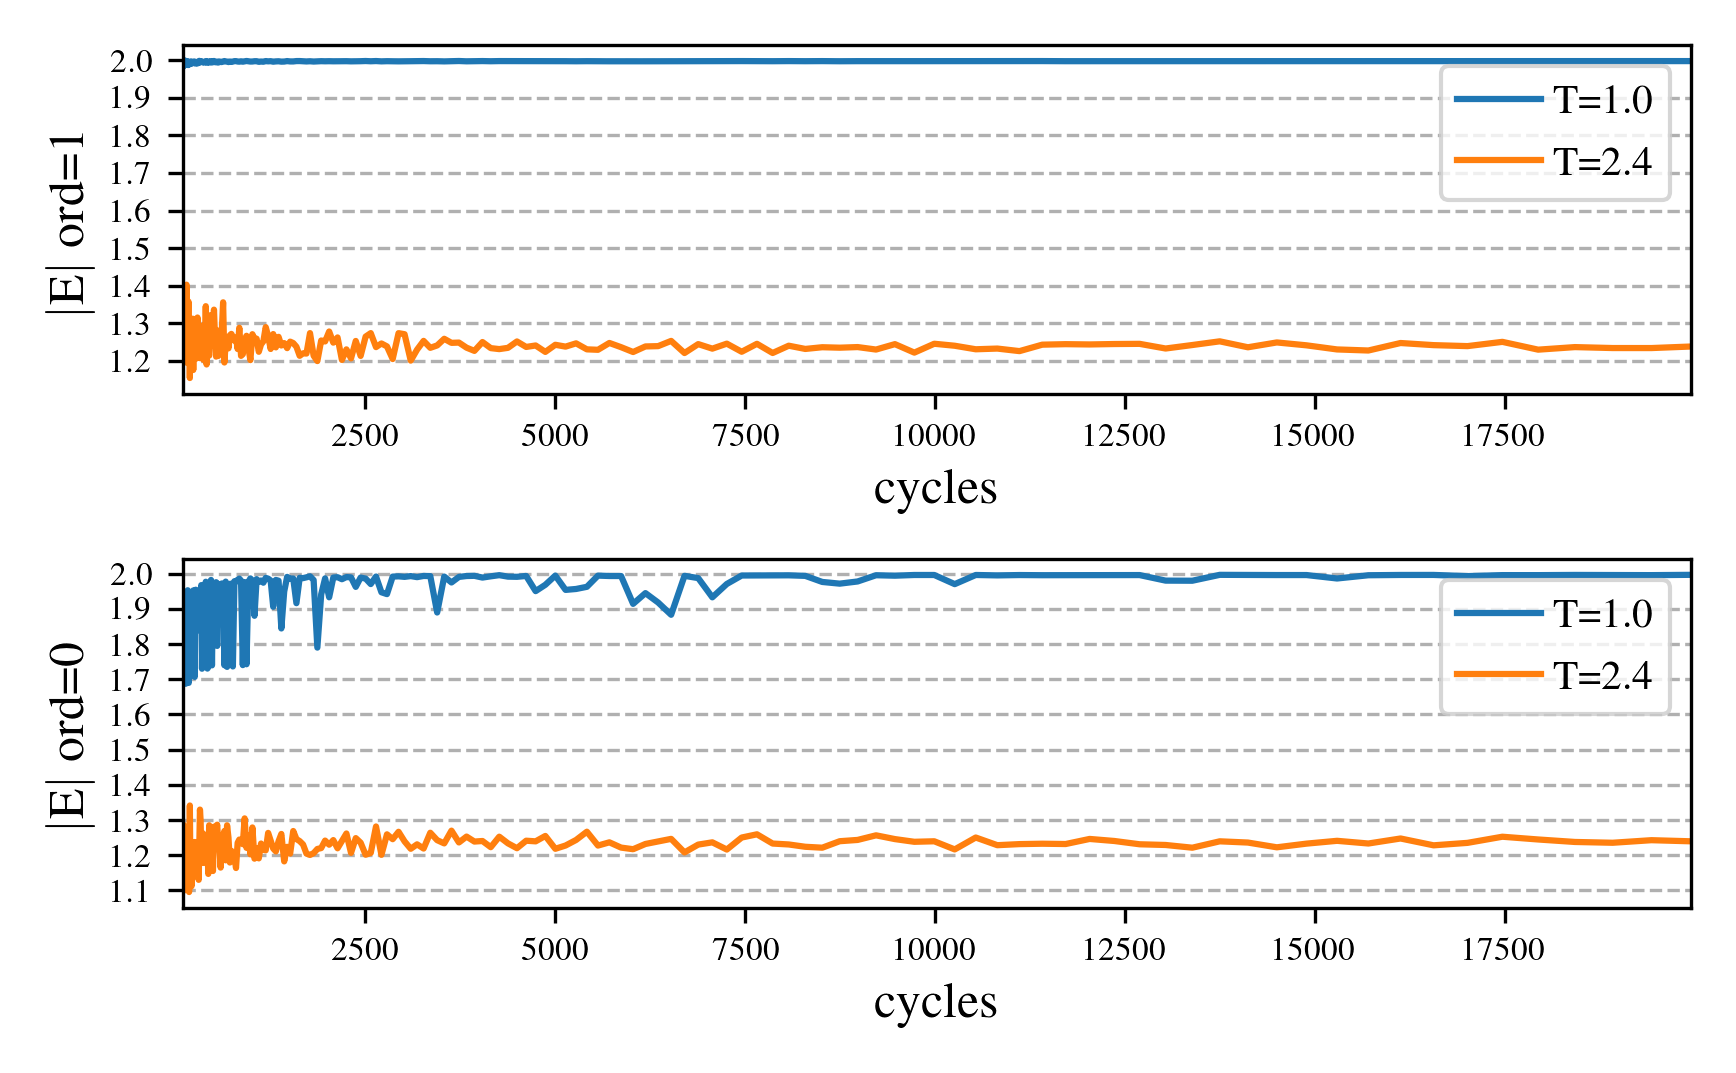
\includegraphics[width=0.8\textwidth]{../figures/equilibrium_E.png}
  \caption{Absolute values of energy for different MC cycles.
  ord refers to the initial configuration of spins. 1=up, 0=random.}
  \label{fig:equi_E}
\end{figure}


\begin{figure}[H]
  \centering
  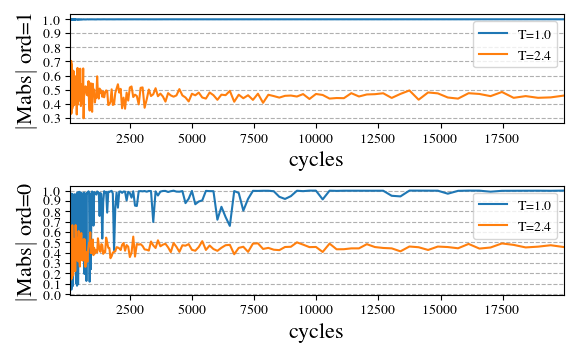
\includegraphics[width=0.8\textwidth]{../figures/equilibrium_Mabs.png}
  \caption{Absolute values of magnetization for different MC cycles.
  ord refers to the initial configuration of spins. 1=up, 0=random.}
  \label{fig:equi_M}
\end{figure}




\begin{figure}[H]
  \centering
  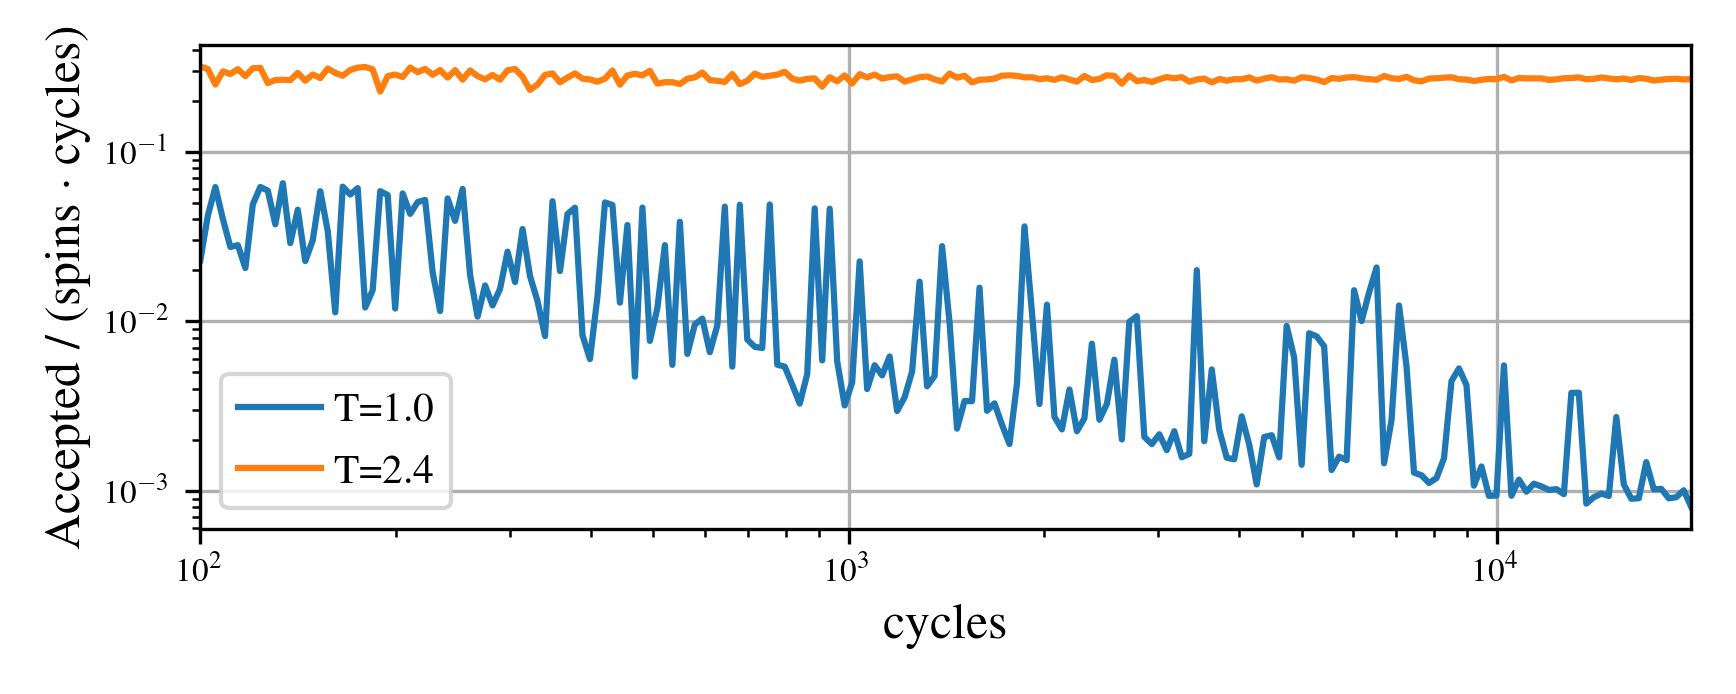
\includegraphics[width=\textwidth]{../figures/accepted.png}
  \caption{Accepted configurations scaled with number of spins and MC cycles.}
  \label{fig:accepted}
\end{figure}

\subsection{Model testing}

Implementation of tests (test\_analytic.py, test\_ising.py) showed that the
analytical solutions was correct down to an absolute error of \num{1e-12}  when
comparing against a brute force method where we created all the possible
microstates.
Testing the ising model against the analytical solutions for a 2x2 grid showed
that we could consistently achieve a relative error of 0.001 with only 100000
Monte Carlo cycles (MCC) for the energy and magnetization. For the heat capacity
and susceptibility we had to increase the MCC to 5 millions and the relative
error tolerance to 0.05.


\subsection{Production runs}

For the production runs (phase\_transitions.py) we parallelized the code with
numba using $@njit(parallel=True)$. We found it easiest to run calculations for
each temperature in parallel, instead of parallelizing the ising model itself.
An unfortunate side effect of this was that we were not able to write to file
after each run of the ising model, so if our run did not finish we would lose
all the results. We also added a script (timings.py) that estimates the time to
run phase\_transitions.py with the given parameters so we did not start too time
consuming runs.

Timings with and without parallelization for small grid sizes showed a speedup
of roughly 3.4 on a laptop with 4 physical cores. The suboptimal speedup might
be related to creation of and writing to the 2d arrays for storing results,
but we did not look deeper into this.
